\chapter{调制识别的深度框架研究}

\section{引言}
目前存在几种较完善的网络,比如包括多层感知机、RNN、CNN及其许多变体以等。
尽管机器学习的目的是提供一种通用的问题解决算法,但目前性能最优的网络模型大部分仍然是对应于特定应用的,
比如谷歌提出的长短期深度神经网络(CLDNN)、Inception模型,微软的残留网络(ResNet)等。 \par
在第三章中,我们基于网络模型的层面,提出了一种不同类型深度模型融合的深度网络框架,并将其应用到无线信号调制识别任务中,
而且取得了一定的性能提升。
在本章中,我们将以LeCun的经典五层网络结构为基准,从网络底层结构单元的层面,
研究当前在各个行业表现优异的不同
的网络底层结构对调制识别性能的影响。\par

\section{网络超参数对调制识别的影响}

\subsection{卷积神经网络}
在大部分现有的深度神经网络中,卷积层成了它们共同的元素。
Lecun成功地将卷基层应用到手写数字识别【】中,以保证特征的平移不变性[8]。
卷积层由$N_f$个卷积滤核组成,每个卷积核通常非常小(1x1到5x5是图像处理中的常见尺寸)。
在传统的DSP应用中,滤波器通常设计得非常宽(很多分支/高阶),而非设计成多层很深的结构(小分支/级联)。
而计算机视觉领域的神经网络的一个明显趋势是建立更深的网络来学习更复杂的功能和层次特征关系[2],[1]。\par
标准卷积层[9]的传递函数在等式3中给出,其中$y_i$是第$i$个滤波器的输出特征图,
$b$和$k$代表学习偏差和滤波器权重参数,$x_i$代表输入激活,$*$ 表示卷积运算,
并且$f(\dot)$表示诸如整流线性单元(ReLU)或S形的(通常非线性的)激活函数:
\begin{equation}
	y_i = f (b_j + \sum_{i}(k_{ij} * x_i))
\end{equation}
深度网络使得可以从原始数据中更容易地学习更复杂的功能,而不是使用相同数量参数的浅层网络[1],[18];
然而,人们普遍认为神经网络中的深度受不稳定梯度的限制,不稳定梯度容易在网络的早期形成梯度爆炸,在后期形成梯度弥散等现象。
近年来,通过在优化器中使用梯度归一化以及新的激活单元(如整流线性单位(ReLU))的提出,
使得我们可以克服或减弱梯度消失以及梯度弥散问题。\par
基准的卷积网络在softmax分类器之前有两个卷积层和一个全连接层。每个隐藏层具有整流线性单元(ReLU)激活函数并使用0.5的$dropout$降低过拟合。\par

\subsection{卷积核数目对调制识别的影响}
我们探究的第一个超参数是卷积核数目,即卷基层的大小,对调制识别的影响。
通过在第三章的探索,我们发现卷积层在第一个卷积层为$1x5$的卷积核大小,第二个卷积层为$2x6$的大小时,有较好的分类性能。
因此,在本小节中,我们继续使用这样的卷积核维度,进行卷积核数目对分类性能影响的探索。\par
由于我们训练神经网络时间成本较高,很难对每一个卷积核数目参数进行遍历,所以我们选择一些有代表性的参数进行试验,主要目的是定性的分析卷积核数目的变化对于分类性能的影响。本论文中我们定义卷积核数目集合$\kappa =\{24, 32, 48, 64, 80, 96, 128, 160, 192\}$,
第一个卷积层与第二个卷积层分别从集合$\kappa$中选取,每层卷积核数目从$24$变化到$193$。
这样两个卷积层的核数目组合共有$|\kappa|^2$种,即网络训练总的遍历次数为$|\kappa|^2$。\par
通过仿真,我们最终得到分类器性能随卷积核数目变化的结果如图\ref{sec:fig_5_1}所示:\par
\begin{figure}[!h]
	\centering
	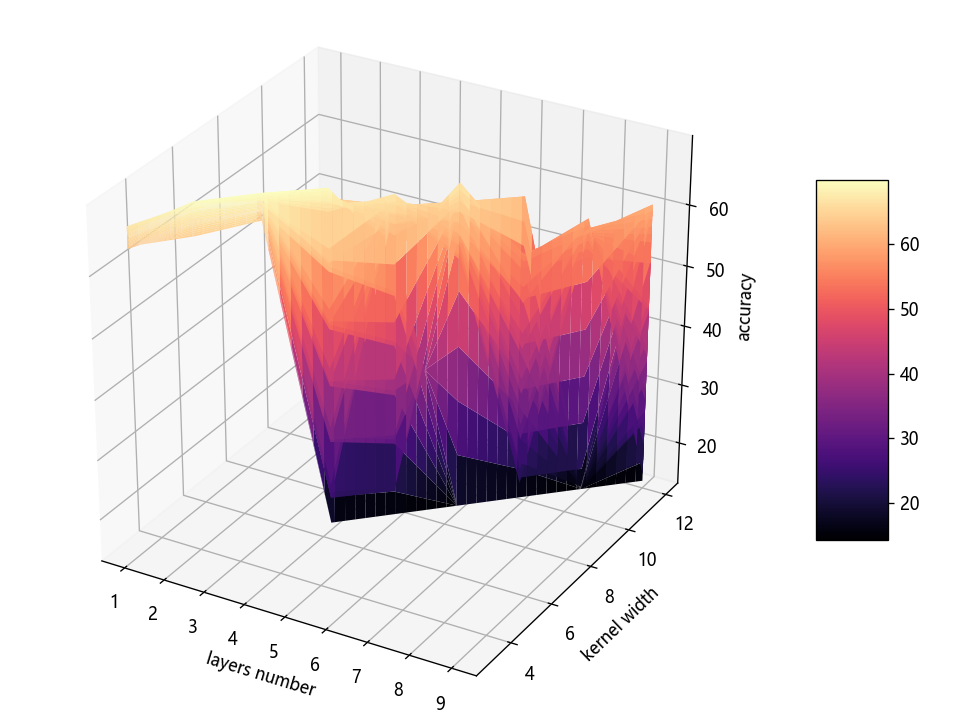
\includegraphics[scale=1.1]{figures/chapter_5/fig_5_1}
	\caption{卷积核数目对分类性能的影响} \label{sec:fig_5_1}
\end{figure}

图\ref{sec:fig_5_1}显示了滤波器数量从24增加到90时,信噪比为0dB时的$7$类信号分类准确率。通过图\ref{sec:fig_5_1}的结果我们可以发现,当第一层和第二层的滤波器数量较小时,分类的准确率处于一个比较低的水准;当第一层和第二层的卷积核数目增加时,分类准确率相应的增加;当第二个卷积层数目增加到64时,网络的分类性能不再随着第一层卷积核数目增加而增加;当第二个卷积层中卷积核的数目大于64时,不管第一层卷积核数目如何变化,分类性能都不能超过最值。通过综合考虑两个卷积层,我们可以发现当第一层卷积核数目为64、第二层卷积核数目为32时,分类器性能达到最优。\par
对于这种现象出现的原因,通过分析,我们认为滤波器数目从网络的复杂度以及网络的特征提取维度两方面影响分类的性能。\par
当卷积核数目很小时,同时由于网络本身的深度较小,因此,受限于卷积特征图数目的限制,特征提取的数目也相应的较少,很难较完整地反映数据本身的特征,分类准确率的上限会出于一个较低值。当卷积核数目增加,相当于我们的特征数目也在相应的增加,这样,网络本身的拟合能力增强,卷积核所提取的卷积特征能更好地反映数据的内在特征,因此,分类性能的上界相应提高,可以获得较好的分类结果。\par
当卷积核的数目增大到一定的程度,网络的拟合能力过强,不仅能够拟合出数据本身的性质,同时将一些异常点也进行了拟合,这就造成了过拟合;同时,由于我们的数据量有限,也很难将网络参数训练到一个较优的水平。因此,我们的分类性能可能会随着卷积核数目的增加而降低。\par

\subsection{卷积核大小对调制识别的影响}
在本小节我们将探究卷积核大小对调制识别性能的影响。根据第三章我们采用的卷积神经网络结构,我们将第一个卷积层的卷积核数目固定在64,将第二个卷积层的卷积核数目固定在32,因为这种情况下网络具有较好的分类性能。\par
我们假设卷积核高度在$0$与$1$之间变化,卷积核的宽度在$3$到$9$之间变化。则总的训练迭代次数为$7 * 7 * 2 * 2$。为了弱化不同网络结构对训练样本$epoch$次数的需求,我们假设$epoch=1000$,这是一个很大的值,但是我们自定义了预停止策略:当每次训练迭代时,$epoch$次数增大10次,而分类性能没有提升,我们则停止本次的训练迭代。整个仿真在我们的硬件平台下大约持续了150小时,结果如图\ref{sec:fig_5_2}所示:\par
\begin{figure}[!h]
	\centering
	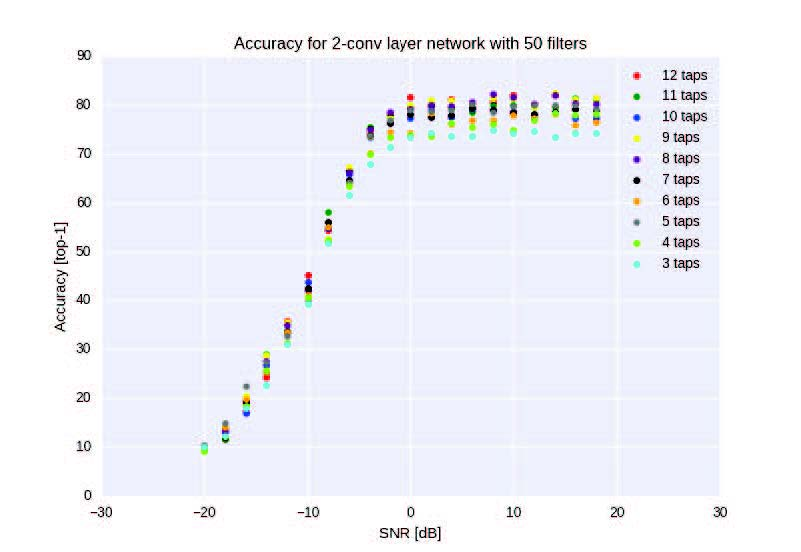
\includegraphics[scale=1.2]{figures/chapter_5/fig_5_2}
	\caption{卷积核大小对调制识别性能的影响}\label{sec:fig_5_2}
\end{figure}
每个卷积层的卷积核尺寸变化的结果表明:1. 对卷积核的宽度而言,整体而言较小的卷积核不如较大的卷积核,但是当卷积的宽度增大到7之后,
分类性能变化很小;2. 对卷积核的高度而言,当第一层卷积核的高度为1,第二层卷积核的高度为2时,我们可以获得相对最优分类性能。\par

通过图\ref{sec:fig_5_2}我们可以发现卷积核宽度为$6-9$时网络的分类性能可以达到一个较高的水准。
这些数目的卷积核宽度相互之间有一定的差异,但是考虑到网络能达到的只是一个局部极小值,
而非全局极小值,我们很难定量的确定到底怎样的卷积核大小是一个最优值。
但是可以确定的是,由于我们的信号样本是128个采样点,而每个样本包含8到16个符号,也就是每个符号占用为$16$或者$8$个采样点。
因此,我们的卷积核宽度为$8$时,每次卷积操作相当于对$1$个符号或$1/2$个符号进行运算,
此时,分类器的性能很有可能达到一个相对较优的水平。\par

对于卷积层的高度而言,由于我们的样本是一个$2\times128$的时间序列,我们可以看成是由两行$128$维的向量组成。
其中,第一行表示信号的实部,第二行为信号的虚部。
这样,我们在利用卷积核对信号进行卷积特征提取时,如果卷积核的宽度为$1$,相当于是在信号的实部进行采样值的卷积运算;
如果卷积核的宽度为$2$表示我本不仅对信号进行实部的运算,同时考虑到了信号的虚部,
这样进行卷积时,可能同时会包含信号的能量信息。
当然,这些只是我们从理论层面的一些分析,具体卷积核维度变化相应于我们信号的哪一些特征,有待后续的进一步研究。
但是,可以确定的是,卷积的操作提取的不仅仅是某些确定的特征,
而很有可能是某些信号特性本身的体现,而且这些卷积特征随着参数的初始化、卷积核的维度变化所表征的含义也是完全不同的。\par

\subsection{网络层数对调制识别的影响}

在本小节我们将探索网络层数对调制识别的影响。
由于我们仅仅是探索卷积层深度对分类性能的影响,而且网络的训练本身是一个非常耗时的过程。
因此,为了降低时间成本并简化分析提供一个定性的结果,我们在本小节中的仿真所有卷积核的大小都为$1x8$,卷积核数目都为32。
在卷积层之后,我们使用单隐层,然后利用softmax分类器作为最后的分类概率。\par
由于网络层次深度对训练数据遍历次数的要求差别很大,我们也应用了与上一小节相同的预停止策略,
在尽量保证准确率的同时提高训练效率。系统的仿真结果如图\ref{sec:fig_5_3}所示。\par
\begin{figure}[!h]
	\centering
	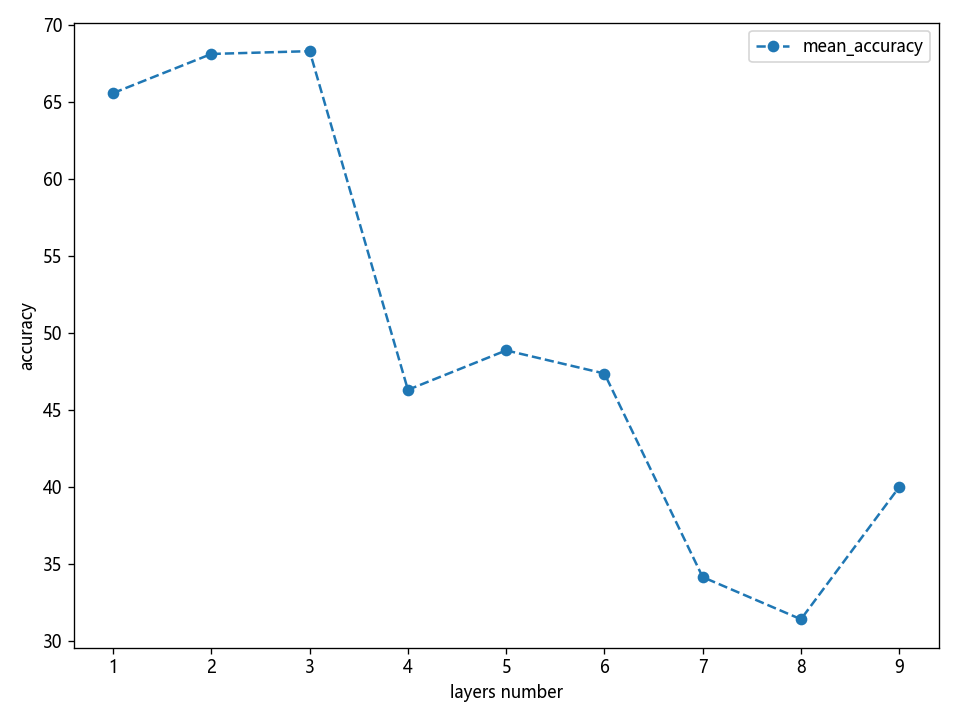
\includegraphics[scale=1.1]{figures/chapter_5/fig_5_3}
	\caption{网络层数对调制识别的影响}\label{sec:fig_5_3}
\end{figure}
我们从卷积层只有$2$层的网络开始,不断增加卷积层深度。
从图\ref{sec:fig_5_3}可以发现,增加卷积层的深度,在卷积层数目小于2时,可以微小地改善分类性能;
当卷积层深度大于2时,改变卷积层的数量在分类准确性方面几乎没有改善。
这表明对于我们的数据而言,没有必要学习更高层次的深度特征。
可能是由于调制数据通常只改变正弦曲线的幅度,频率或相位,因此数据的原始的复杂度不高。\par

然而,令我们意外的是,添加更多的卷积层似乎并不能在低信噪比下提高分类器的性能。
这可能是由于在低信噪比下,由于噪声能量占比过高,覆盖了调制数据本身的特性,
而深度网络更多的是对加噪之后的数据的数值特性进行特征提取,对于统计量、循环谱等特性并没有涉及,
因此低信噪比下分类器的识别性能并没有得到提高。\par

\section{现有的网络架构}
LeNet主要是用于识别10个手写数字的,但其具有较简单的网络底层结构,对于复杂数据识别效果较差。自2016年ImageNet竞赛之后,深度学习在之后大放异彩,下图是近几年主流的深度框架(AlexNet、VGG、GoogLeNet、ResNet)的比较。\par
\begin{figure}[!h]
	\centering
	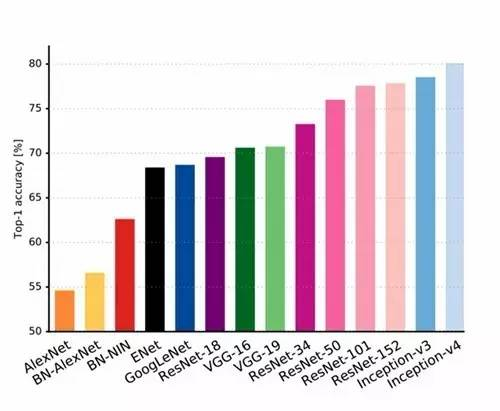
\includegraphics[scale=0.5]{figures/chapter_5/fig_5_4}
	\caption{不同网络结构ImageNet竞赛top1准确率}\label{sec:fig_5_4}
\end{figure}
AlexNet相比传统的CNN的改进主要在数据增强、dropout、池化、ReLU函数等,相较于我们提出的CNN基础框架没有本质上的区别。
而VGG主要的改进是网络深度的改进,对我们的调制数据而言,网络深度的增加并不能带来模型性能的提升。
因此,本文中我们对其影响并不作研究,而是主要对几个主流框架GoogLeNet、ResNet、CLDNN的底层结构进行改动适应调制信号的维度,
并降低网络深度,观察不同的底层网络结构对调制识别的影响。

\subsection{GoogLeNet}
GoogLeNet相较于CNN主要的创新在于提出了Inception结构,这是一种底层的网络结构,其类似于卷积核一样,是一种网络组成的单元。
它可以提高网络深度和宽度,并能够将不同规模的特性推广到一般管理复杂性。
Inception一直在不断发展,目前已经发展到$v4$版本,对于我们的调制识别应用场景,
经过修改后基本的网络结构如图\ref{sec:fig_5_5}所示:\par
\begin{figure}[!h]
	\centering
	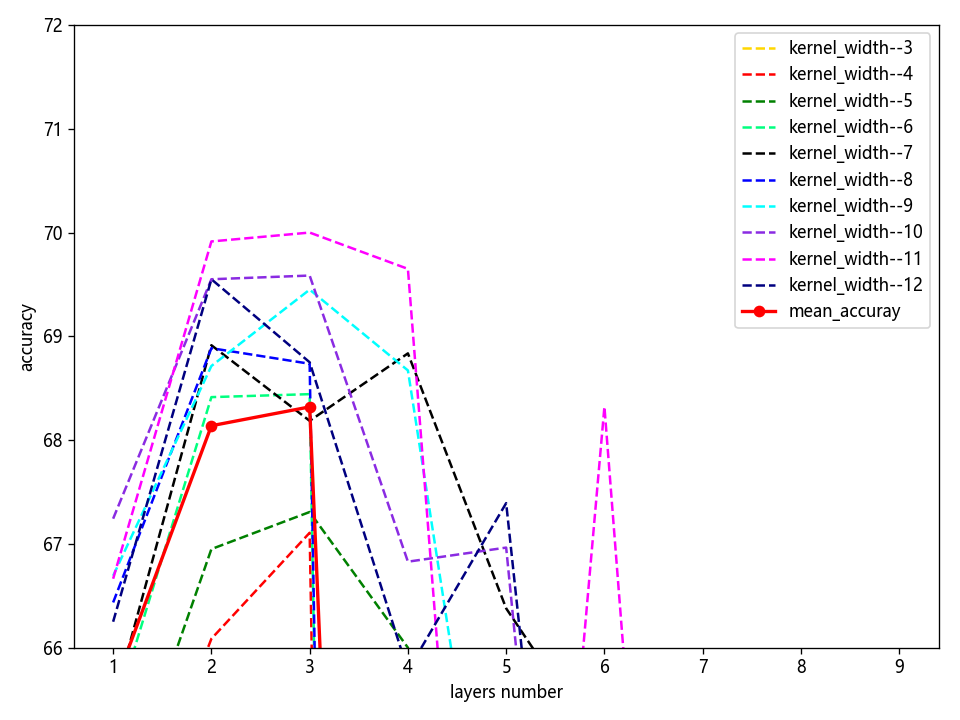
\includegraphics[scale=0.8]{figures/chapter_5/fig_5_5}
	\caption{InceptionModel}\label{sec:fig_5_5}
\end{figure}
每个Inception模块(如图\ref{sec:fig_5_5}所示)包含四条并行路径,输出是四个并行输出的串联,
用了Inception结构之后整个网络结构的宽度和深度都可扩大。
第一条路径是一组对选定信息转发的$1\times1$卷积核,它只是简单地向前传递信息而不进行变换,
可以使选择性信息高速前向传播。
第二和第三条通道首先是$1\times1$卷积,接着是一组$1\times3$和$1\times8$卷积以提供多个宽度的特征检测。
最后一条并行通道,首先是一个3x3池化层,接着是1x1卷积。\par
我们在特征提取层中使用了两层适应性重构后的Inception网络,其中第一层包含32个Inception结构,第二层包含16个Inception结构。
这样,我们可以保证在尽量不提高网络深度和宽度的情况下,学习数据的不同维度特征。\par

\subsection{残差网络}
残差网络(ResNet)的提出本质上是要解决层次比较深的时候无法训练的问题。
使用跨层转发信息的体系结构是一种增加网络深度的有效方法,
微软凭借ResNet的网络结构增加网络层深度至152层并赢得ImageNet 2015的冠军[4]。
这种借鉴了Highway Network思想的网络相当于在主干网络之外开通一个特殊通道使得输入可以直达输出。
图\ref{sec:fig_5_6}展示了ResNet的基本结构:\par
\begin{figure}[!h]
	\centering
	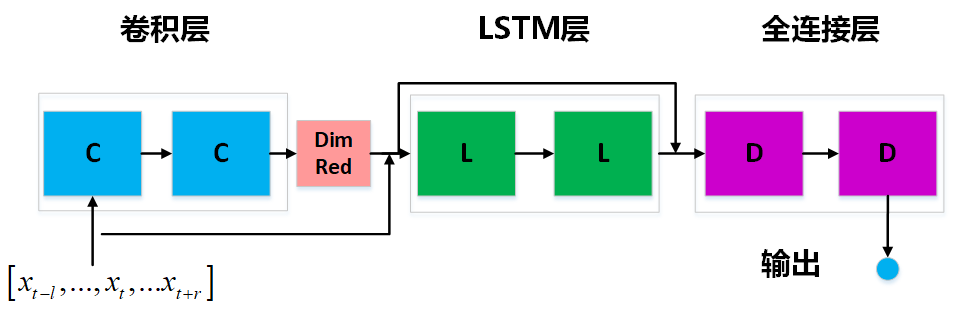
\includegraphics[scale=0.6]{figures/chapter_5/fig_5_6}
	\caption{残差网络结构}\label{sec:fig_5_6}
\end{figure}
如图\ref{sec:fig_5_6}所示,,$x$是网络的输入,主干网络为输入信号$x$经过不同的网络层后向传播;
同时,ResNet也会将一层的输出添加到更深层的两层输出中。
其中$H(X)$是某一层原始的的期望映射输出,而优化的目标由原来的拟合输出$H(x)$变成输出和输入的差$H(x)-x$,
由于ResNet的信息转发迫使网络学习残差函数进而学习数据的特征,因此这样的网络结构被称之为残差网络。\par
ResNet的作者认为消失梯度可以通过广泛采用的归一化技术来解决,而深度网络的深度则受限于深度网络的训练复杂度,
而残差网络正可以通过额外的信息转发通道,弱化网络深度对训练复杂度的影响。\par

由本章第二小节得到的结论,网络的深度并不是我们调制性能限制的主要因素。
因此,我们在ResNet调制识别网络的设计时,仅仅考虑到使用五个层的简单网络,每隔两层进行信息转发,
来探索ResNet的网络结构是否能提高调制识别的准确率。


\subsection{卷积长短期深度神经网络}

卷积长短期深度神经网络(Convolutional Long short-term Deep Neural Networks,CLDNN)是语音处理的一种算法,
它可以在原始时域波形上进行运算。
该体系结构使用两个卷积层,随后是两个由长期短期内存(LSTM)单元组成的循环层。LSTM是一种常见的经常性网络架构,由几个门控制,历史维持多久[5]。 CLDNN也可以具有绕过层的连接,旨在为提取的功能提供更长的时间上下文。例如,原始CLDNN在LSTM层之前转发具有卷积层输出的原始样本[11]。
受使用专业知识指导卷积网络和CLDNN等网络体系结构的启发,我们尝试使用卷积网络,我们将其称为卷积匹配滤波器。相当简单的想法是采用典型通信接收器的通用架构,并构建具有类似部分的神经网络架构。通信接收机有一个滤波器(通常与传输的脉冲或波形匹配),同步器和采样器。通常,前置滤波器抽取每个符号的少量采样,用于执行相移以找到最佳采样点的同步器。采样器然后切片到比特或发出音频用于模拟调制。与此类似的神经网络体系结构是一个卷积层,后面跟着一个LSTM。

作为我们测试的最终架构添加了用于建模时间特征的LSTM。由于调制基带数据是时间序列,因此预计这将是一个重大改进。在LSTM层之前,我们测试了两层和三层卷积和CLDNN型架构,其中有和没有前向连接。我们发现前向连接是原始波形和卷积输出的连接,如图2所示。与其他架构相比,分类精度更高,梯度下降更稳定。使用会创建类似前面描述的卷积匹配滤波器检测器的体系结构的合并层不利于分类。
为了进一步理解什么限制了分类的准确性,我们看一下图1所示的CLDNN的混淆矩阵。 8.有两个主要的混淆领域。一个在模拟调制之间,另一个在高阶QAM之间。模拟调制将很难解决,但是QAM可以通过更好的同步和减少信道损伤来改善。
对CLDNN在每一层学习的内容有直觉,对指导未来的工作很重要。为此,我们绘制了一些滤波器抽头的时间和频率表示。对于频率响应,滤波器抽头用零填充100个零点以获得128点FFT。图图9a和图10a示出了来自第一层的两个选择滤波器。专家的眼睛看起来并不特别熟悉时域表示;然而频率响应确实显示了整形的低通滤波器。未示出的其他滤波器具有频率选择性组件,DC阻断器和类似sinc的频谱形状。



受使用专业知识指导网络体系结构(如卷积网络和CLDNN)的启发,我们尝试使用卷积网络,我们将其称为卷积匹配滤波器。 相当简单的想法是采用典型通信接收器的通用架构,并构建具有类似部分的神经网络架构。 通信接收机有一个滤波器(通常是采样器),通常前置滤波器抽取每个符号的少量采样,用于执行相移以找到最佳采样点的同步器,然后采样器切片成比特或发射音频以进行模拟调制 。与此类似的神经网络体系结构是一个卷积层,后面跟着一个LSTM。\par

作为我们测试的最终架构添加了经常性网络层,即那些由LSTM单元组成的层,用于对时间特征进行建模。 这种方法广泛用于时间序列应用,我们预计调制基带时间序列可能同样适用。 我们测试了两层和三层卷积,然后在CLDNN类型体系结构中重复出现层,在重复层之前有和没有前向/旁路连接。 我们发现前向连接作为原始波形和卷积输出的连接,如图8所示,与其他体系结构相比,分类精度更高,梯度下降更稳定。 使用会创建类似前面描述的卷积匹配滤波器检测器的体系结构的合并层不利于分类。\par
\begin{figure}[!h]
	\centering
	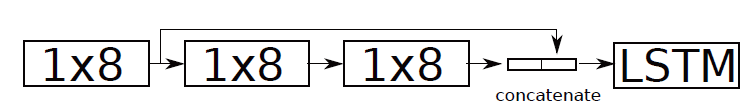
\includegraphics[scale=1]{figures/chapter_5/fig6}
	\caption{用于RF数据的CLDNN体系结构。 在进入LSTM之前,第一个1x8卷积层的输出与三个1x8卷积层的输出级联。}
\end{figure}

为了进一步理解什么限制了分类精度,我们查看了图10中所示的CLDNN的混淆矩阵。有两个主要混淆领域。 一个在模拟调制之间,另一个在高阶QAM之间。 模拟调制将很难解决,但是QAM可以通过更好的同步和减少信道损伤来改善。\par
\section{结果及分析}

\subsection{神经网络训练}

网络的超参数(如学习速率,每层过滤器/特征映射的数量,过滤器大小以及某种程度上的层数)都会影响网络规模并且难以优化。 最近的研究尝试将超参数优化为可以用反向传播和梯度下降(如网络权重和偏差)进行训练的常规参数。 对于这项研究,我们忽略训练超参数,并使用adam优化器[6],它提供梯度归一化和动量,降低超参数的重要性,如学习率。

在工作的指导下,深度比特征图的数量更重要[2],我们将建立一个类似于无线电卷积调制网络[13]中使用的基线卷积网络。 我们的第一步是调整每个滤波器的滤波器数量和抽头数量,并将其视为不重要的超参数,用于余下的实验以测试不同架构对RF数据的适用性。


\subsection{网络参数}

网络的超参数(如学习速率,每层过滤器/特征映射的数量,过滤器的大小以及层的数量)都会影响网络规模,难以优化。
最近的研究尝试将超参数优化为可以用反向传播和梯度下降(如网络权重和偏差)进行训练的常规参数。
对于这项研究,我们忽略训练超参数,并使用adam优化器[6],它提供了梯度归一化和动量,降低了像学习率这样的超参数的重要性。
在工作的指导下,深度比特征图的数量更重要[2],我们将建立一个类似于无线电卷积调制网络[13]中使用的基线卷积网络。
我们的第一步是调整每个滤波器的滤波器数量和抽头数量,并将其视为不重要的超参数,用于剩余的实验,
以测试不同架构对RF数据的适用性。\par

我们使用RadioML2016.10a数据集[12]作为评估调制识别任务的基础。
目标是使用128个样本的复数(基带I / Q)时域矢量来识别11种可能类别中的调制方案。 
128个样本以2x128向量馈入网络,其中复数时间样本的实部和虚部被分开。
该数据集使用功率延迟分布,频率选择性衰落,本地振荡器偏移和加性高斯白噪声以及这些效应的细节[12]。
数据集标有调制类型和SNR地面实况。
我们使用全SNR的top-1分类精度作为单个数字基准,并且比较技术显示SNR高于1的精度。
所有模型和培训均使用Kera深度学习库,使用Nano GTX 1070 GPU使用theano后端。
我们从一个类似于CNN2网络的网络开始[13]。
这是选择的基线,因为[13]的结果显示专家方法的显着改进;任何进一步的改进都应该被认为是最先进的。
主要区别在于我们将在每个图层上使用尺寸为1xtaps的nfilt滤镜。
我们将做一个简单的超参数优化\par

\begin{enumerate}
	\item[a.] 为RF调制识别找到最佳滤波器数量和滤波器大小
	\item[b.] 从网络深度和过滤器大小的其他领域获得测试假设
\end{enumerate}


\subsection{CLDNN}

\begin{figure}[!h]
	\centering
	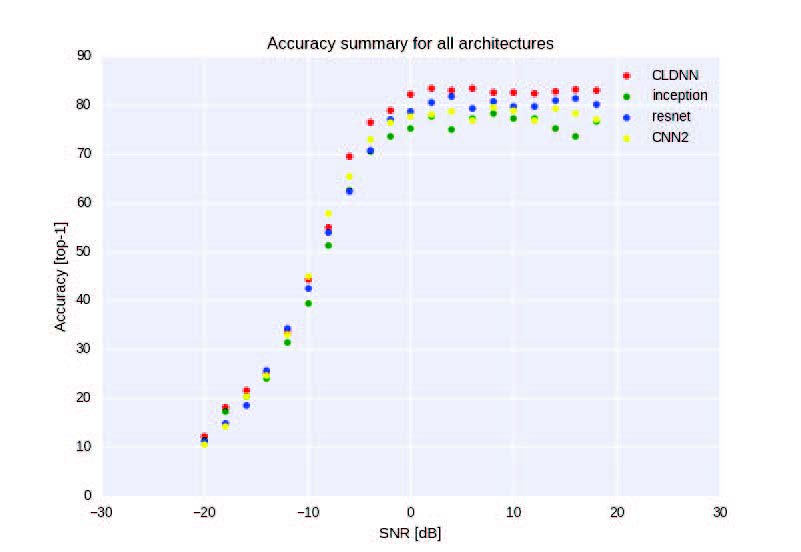
\includegraphics[scale=1]{figures/chapter_5/fig7}
	\caption{CLDNN的信噪比始终优于其他网络架构,信噪比高于-8dB}
\end{figure}

为了进一步理解什么限制了分类的准确性,我们看一下图8所示的CLDNN的混淆矩阵。有两个主要的混淆领域。一个在模拟调制之间,另一个在高阶QAM之间。模拟调制将很难解决,但是QAM可以在更好的同步和减少信道损伤的情况下得到改善。\par

\begin{figure}[!h]
	\centering
	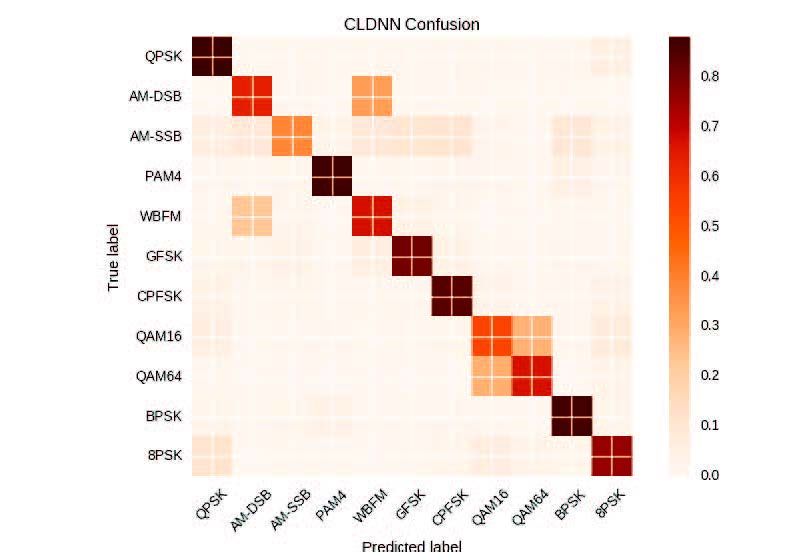
\includegraphics[scale=1]{figures/chapter_5/fig8}
	\caption{CLDNN的全SNR混淆矩阵显示了模拟调制和高阶QAM之间单独混淆之间最混乱的问题。}
\end{figure}

对CLDNN在每一层学习的内容有直觉,对指导未来的工作很重要。 为此,我们绘制了一些滤波器抽头的时间和频率表示。 对于频率响应,滤波器抽头用零填充100个零点以获得128点FFT。图 图11a和12a示出了来自第一层的两个选择滤波器。 专家的眼睛看起来并不特别熟悉时域表示; 然而频率响应确实显示出成形的低通滤波器。 未示出的其他滤波器具有频率选择性组件,DC阻断器和类似sinc的频谱形状。\par
\begin{figure}[!h]
	\centering
	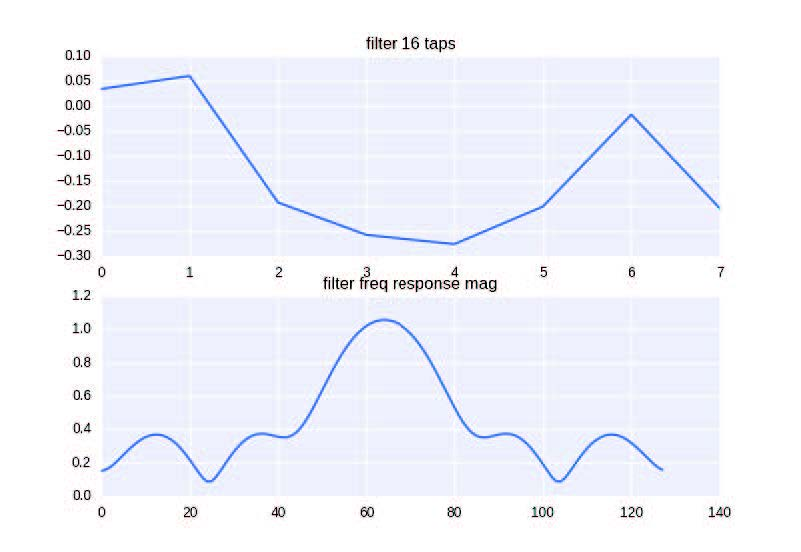
\includegraphics[scale=1]{figures/chapter_5/fig9_a}
	\caption{我们训练的CLDNN的第一卷积层中滤波器的时间和频率幅度表示。。}
\end{figure}
\begin{figure}[!h]
	\centering
	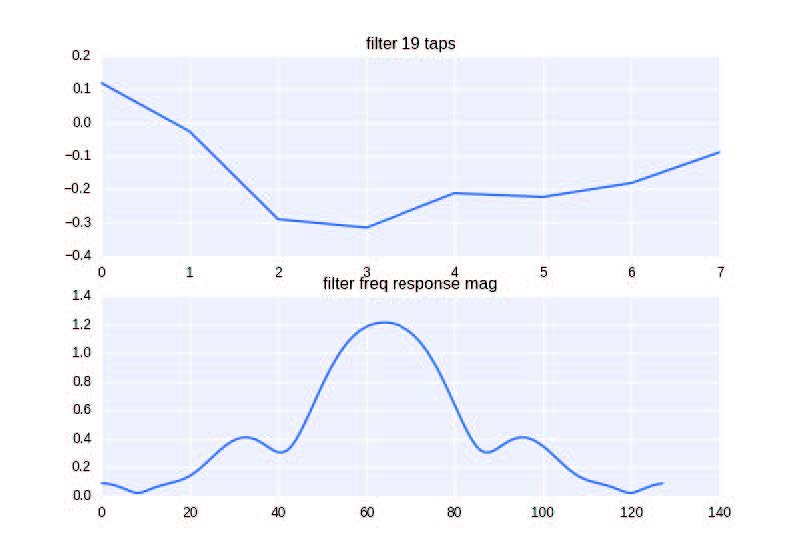
\includegraphics[scale=1]{figures/chapter_5/fig10_a}
	\caption{我们训练的CLDNN的第一卷积层中滤波器的时间和频率幅度表示。。}
\end{figure}
另一种可视化这些滤波器的方法是将随机数据应用于它们,并对特定滤波器的输出执行梯度上升,该滤波器将收敛到最能激活卷积神经元的数据上[11]。 选定的两个过滤器的结果如图2所示。 11b和12b。 所得到的载体看起来有点像粗PSK和FM / FSK调制到专家眼睛。 由于模拟的信道模型,矢量还显示出存在于我们的数据集中的一些恒定的相位旋转。 需要注意的是,选择这两种过滤器可视化并非所有过滤器都对专家有意义。\par

\begin{figure}[!h]
	\centering
	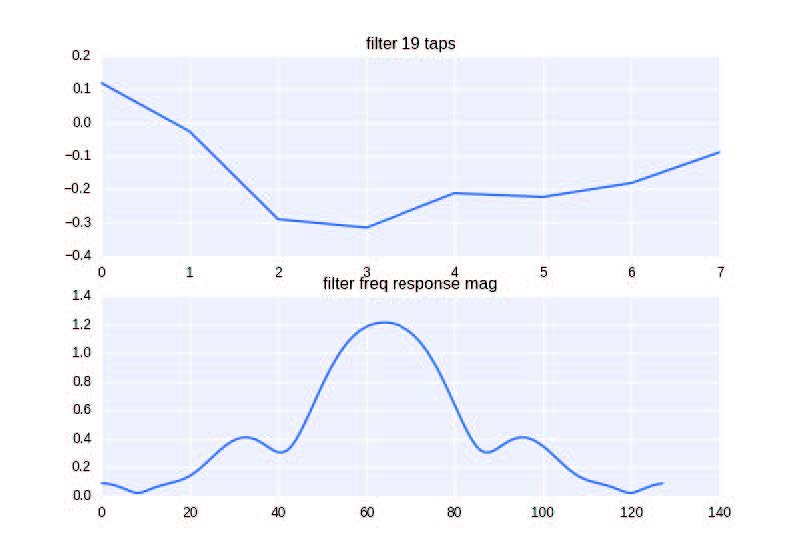
\includegraphics[scale=1]{figures/chapter_5/fig9_b}
	\caption{随机数据训练最大程度地激活过滤器,看起来像BPSK。}
\end{figure}

\begin{figure}[!h]
	\centering
	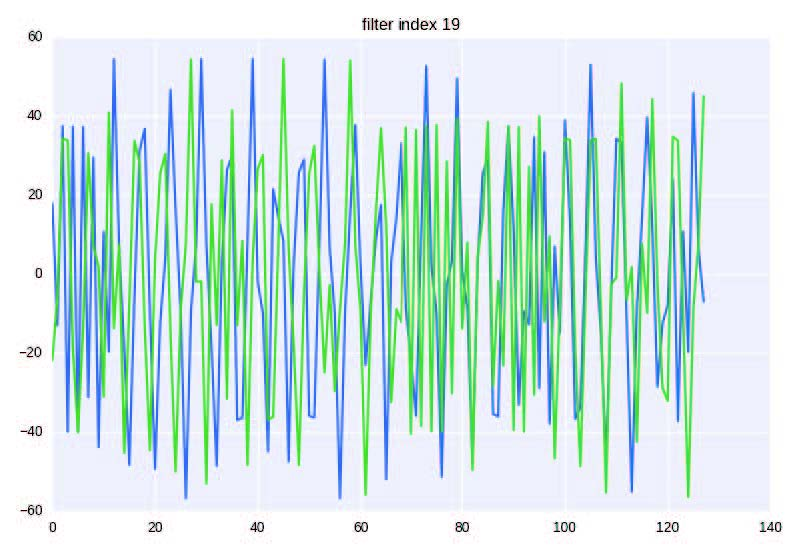
\includegraphics[scale=1]{figures/chapter_5/fig10_b}
	\caption{训练最大程度激活滤波器的随机数据,这看起来像FM或FSK调制。}
\end{figure}
改变卷积层的数量在分类准确性方面几乎没有改善。图1显示了这项任务对信噪比的精确度。这表明我们的网络没有更多的特征深度可以学习。由于调制数据通常只改变复数正弦曲线的幅度,频率或相位,因此数据的起始层次不高;然而,令人惊讶的是,添加更多的卷积层似乎并不能在较低的信噪比下帮助降低噪声的影响。
尽管添加更多卷积层不会提高分类准确性并不奇怪,但令人惊讶的是分类和丢失在2或3卷积层快速提高。最初的研究结果表明,较深的网络会导致较高的训练损失,这表明较高的训练难度而不是过度训练。图4显示,我们的超参数优化CNN和9层残留网络达到了相似的损失,验证损失和准确性,但未显示;然而,剩余网络在更少的时期学习。我们还试验了5-9层的残留网络,它们都具有相似的性能和训练时间。这与我们对普通CNN深度的超参数搜索相结合,表明我们不受无线电学习任务网络深度的限制,尽管我们受到纯粹CNN架构可以学习的功能的限制。

Inception结构在我们的实验中并没有改进无线信号调制分类的识别准确率。网络中1-4个启动模块的结果并没有显示出我们的超参数优化CNN的改进。 同样,这表明我们不受深度的限制,也不受限于滤波器的规模。\par

\section{本章小结}
深度神经网络在无线电领域的性能似乎不受网络深度的限制。 虽然我们的实验将调制识别作为基准任务,但我们期望其他无线机器学习任务能够使用类似的网络架构。 无线电任务深度学习的进一步发展可能来自改进的训练方法和网络架构,这些架构可以学习转换射频数据以消除无线信道的影响,而这些神经网络架构并非为此设计的。 目前正在探索的一个例子是使用空间变换来均衡和同步输入波形[14]。\par

这些实验还着重于名义上带宽归一化的数据集,这是对从真实无线电传输中捕获的信号的不良假设。 将来在实际应用中使用的网络需要学习对信号进行重新采样以获得带宽规格化,或者学习许多带宽的特性。 可重新采样,同步和消除非线性信道失真的网络都是该领域未来令人兴奋的工作。 我们相信,随着无线电环境变得越来越复杂,将调制,多调制协议的不同时间行为和多个无线电发射机组合在一个频带内进行互操作,这些深层网络中的层次结构的许多概念将越来越重要,使我们的网络 可以有效地应对复杂性,正如在复杂的多物体场景中的视觉域中所显示的一样。\par